\documentclass{book}
\usepackage[10pt]{extsizes}
\usepackage[T1]{fontenc} % higher quality font encoding
\usepackage[sfdefault]{universalis} % load the font and set it to default
% Language setting
% Replace `english' with e.g. `spanish' to change the document language
\usepackage[english]{babel}

\usepackage{titlesec}
\titleformat{\chapter}{\normalfont\huge\bfseries}{\thechapter}{1em}{}

% Set page size and margins
% Replace `letterpaper' with `a4paper' for UK/EU standard size
\usepackage[a4paper,top=2cm,bottom=2cm,left=3cm,right=3cm,marginparwidth=1.75cm]{geometry}

% Useful packages
\usepackage{amsmath}
\usepackage{graphicx}
\usepackage[colorlinks=false]{hyperref}
\usepackage{subcaption}
\usepackage{wrapfig}
\usepackage{tcolorbox}

\newcommand{\infobox}[1]
{
    \begin{tcolorbox}[colback=orange!5!white, colframe=orange!75!black]
        \begin{minipage}{0.1\textwidth}
            \centering
            
\includegraphics[width=\textwidth]{../Images/attention-43524-svgrepo-com.png}
        \end{minipage}
        \hfill
        \begin{minipage}{0.85\textwidth}
            #1
        \end{minipage}
    \end{tcolorbox}
}

\usepackage{array}
\newcolumntype{P}[1]{>{\centering\arraybackslash}p{#1}}

\usepackage{fontspec}
\usepackage{lilyglyphs}

\usepackage[backend=biber]{biblatex}
\addbibresource{refs.bib}

\title{Strings? Why not!}
\author{Enzo Evers}

\begin{document}
\maketitle

\tableofcontents

\part{Guitar}
\chapter{Music notation}

\section{Music notation anatomy}

\subsection{Note names}

You have already seen the music staff from \ref{fig:ukulele_music_note_names_on_staff} in the previous exercises. However, the meaning of it was not explained yet.

The letters A-G on the staff show which line on the staff has which note value. The notes that are in between the lines nicely spell out "FACE", making it easy to remember. The Note that are on the lines can be remembered with the mnemonic "\textbf{E}very \textbf{G}ood \textbf{B}oy \textbf{D}oes \textbf{F}ine". But another important thing to see is that the notes go up alphabetically (starting again with A after G). 

The most left symbol (\clefG) is called the G clef. Note that the curl of the G clef is on the line of the G note. 

The vertical line in the middle indicates the start/end of a new measure. and the thinner vertical line in at the end indicates the end of the piece.

\begin{figure}[h]
	\centering
	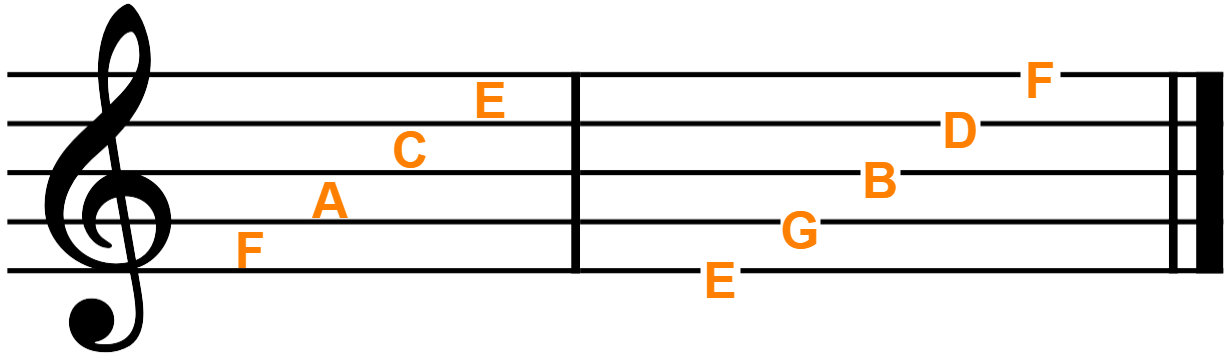
\includegraphics[width=0.6\textwidth]{../../Images/MusicNotation_MeasureNoteNames.png}
	\caption{Note names on the staff in two measures}
	\label{fig:ukulele_music_note_names_on_staff}
\end{figure}

\newpage

\subsection{Time signatures}

So far we have also only seen one type of note. The quarter note. However, there are more. See \ref{fig:ukulele_note_duration_basic}. The \lilyTimeSignature{4}{4} means that there can fit 4 (top number) quarter notes (bottom number) in a measure. 

\begin{figure}[h]
	\centering
	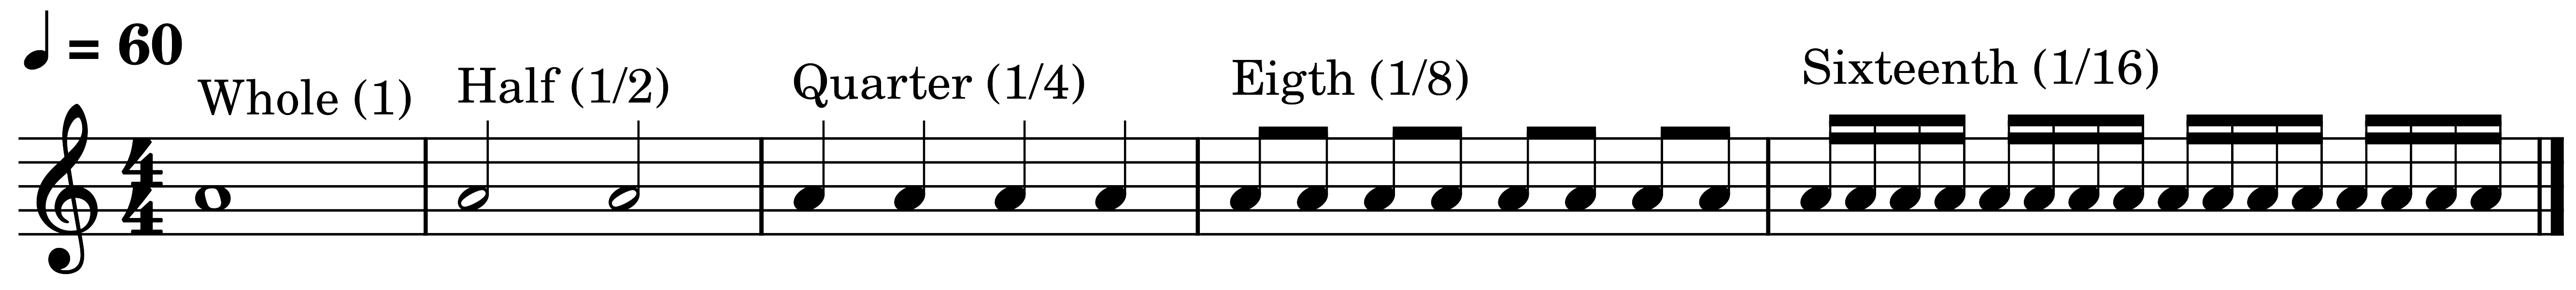
\includegraphics[width=\textwidth]{../../MuseScore/Ukulele/MusicNotation/NoteDurations_Basic.png}
	\caption{Note duration}
	\label{fig:ukulele_note_duration_basic}
\end{figure}

\textbf{Important}: A whole note (\wholeNote) equal 4 quarter notes (\quarterNote). It does \textbf{not} equal a whole measure. \newline

There are also other time signatures. But they all have the meaning. The top value indicated how many notes of the bottom number's duration fit in a measure. So a \lilyTimeSignature{3}{4} time signature can fit 3 quarter notes per measure. And a \lilyTimeSignature{6}{8} time signature can fit 6 eight notes per measure. Note that \lilyTimeSignature{3}{4} and \lilyTimeSignature{6}{8} actually indicate the same duration per measure, but they indicate a different feel. This is indicated in \ref{fig:time_signatures}

In \ref{fig:ukulele_time_signatures} you also see a new duration notation. In the first measure with \lilyTimeSignature{6}{8} timing, there are dots next to the notes (\quarterNoteDottedDown). This means that the note has a duration of 1.5x its original duration.

\begin{figure}[h]
	\centering
	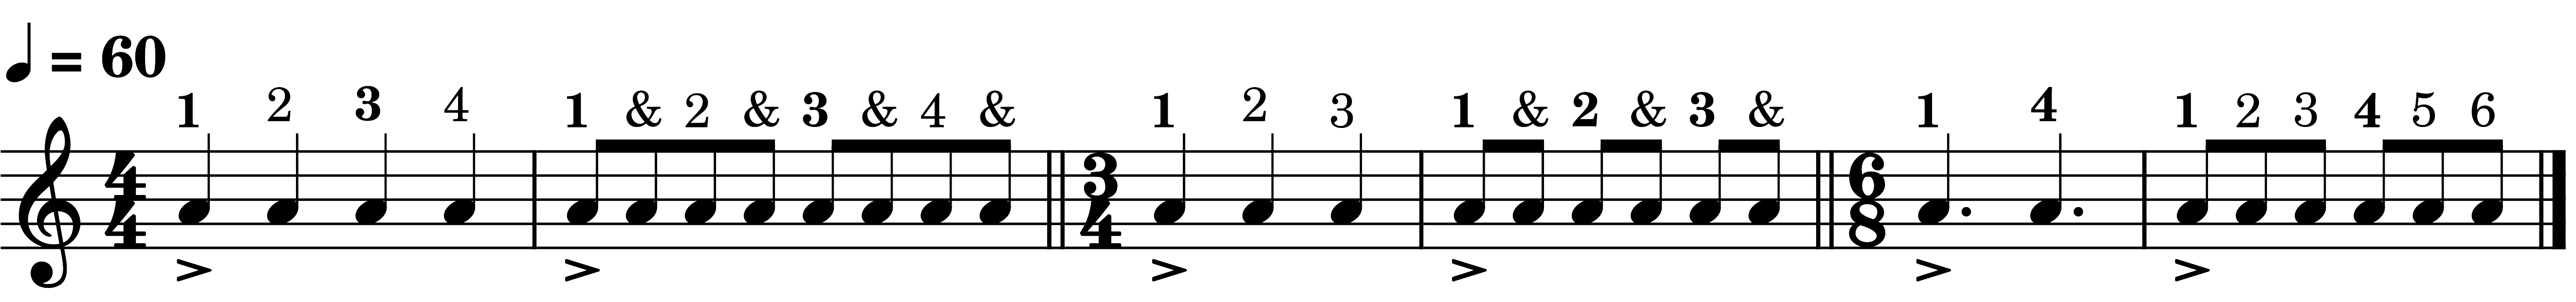
\includegraphics[width=\textwidth]{../../MuseScore/Ukulele/MusicNotation/TimeSignature.png}
	\caption{Time signatures}
	\label{fig:ukulele_time_signatures}
\end{figure}

\newpage

\subsection{Exercise}

In preparation to play the well-known "Tetris" tune, the notes from \ref{fig:ukulele_notes_for_tetris_first_part} should be learned.

\begin{figure}[h]
	\centering
	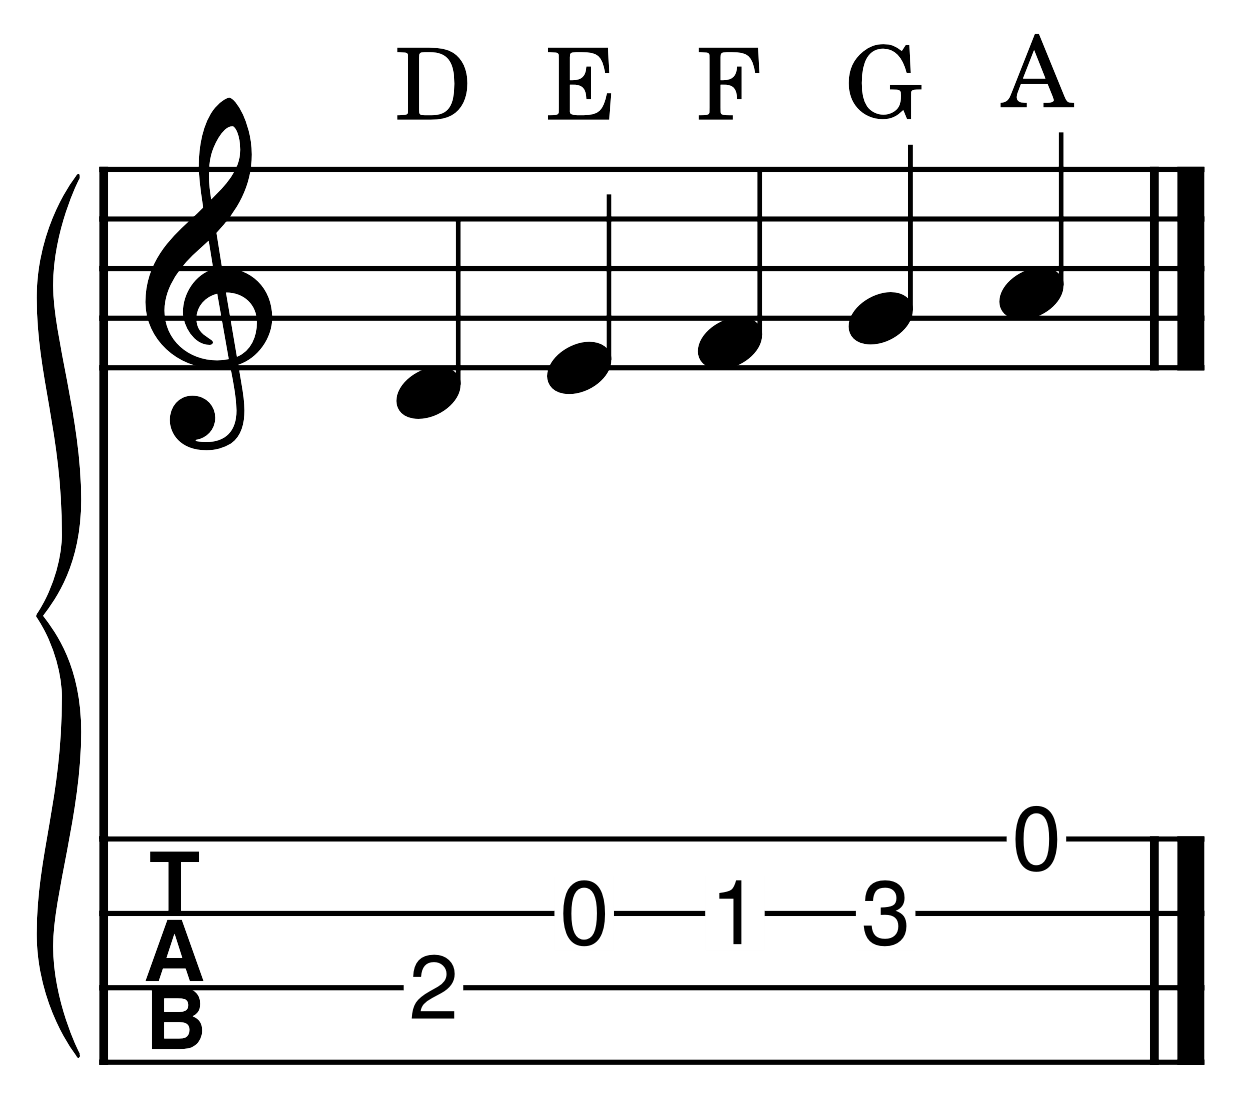
\includegraphics[width=0.25\textwidth]{../../MuseScore/Ukulele/UkuleleNotesUsedInTetrisFirstPart.png}
	\caption{Notes used for the first part of the Tetris tune}
	\label{fig:ukulele_notes_for_tetris_first_part}
\end{figure}

In \ref{fig:ukulele_tetris_simple_first_part} the first part of the Tetris tune is written. This time no TABs are shown. This exercise has 4 different note durations and 5 different notes pitches.

\begin{figure}[h]
	\centering
	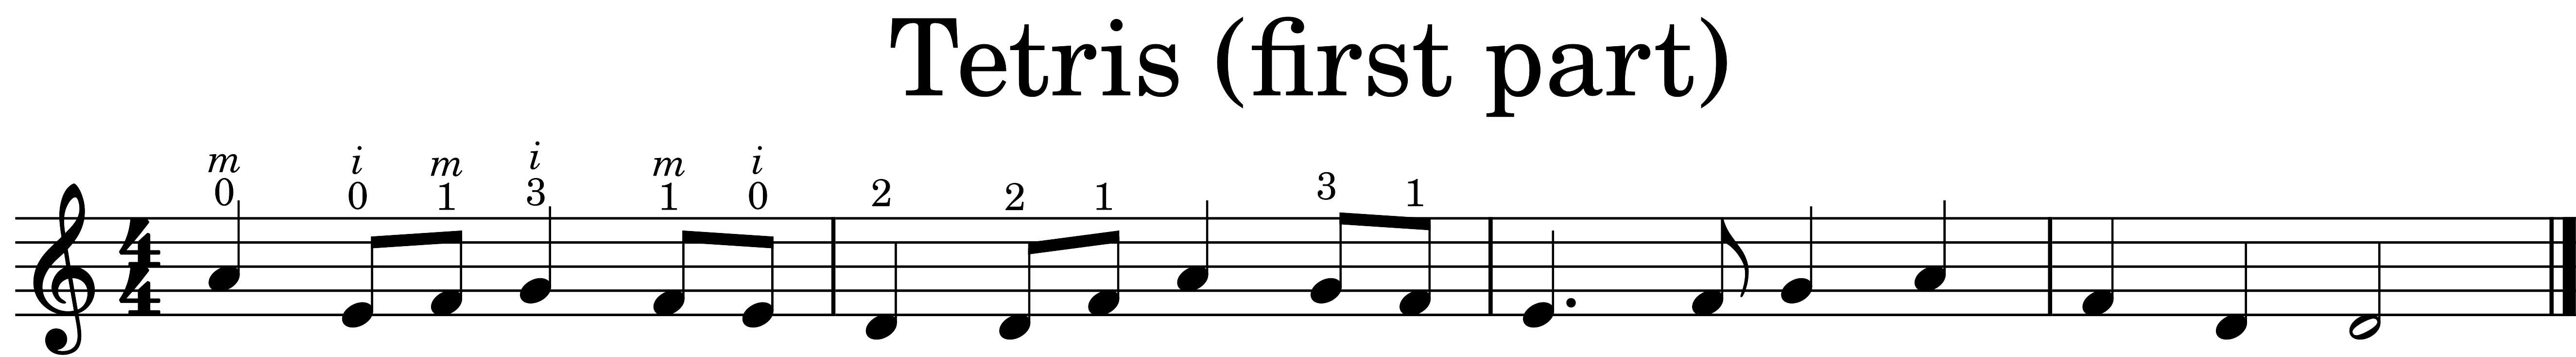
\includegraphics[width=\textwidth]{../../MuseScore/Ukulele/UkuleleTetrisSimpleFirstPart.png}
	\caption{First part of the Tetris tune}
	\label{fig:ukulele_tetris_simple_first_part}
\end{figure}


\infobox{The "Tetris" tune is actually derived from a Russian folk song called "Korobeiniki", which is based the a similar named poem written by Nikolai Nekrasov.}
\newpage
\chapter{Music notation}

\section{Music notation anatomy}

\subsection{Note names}

You have already seen the music staff from \ref{fig:ukulele_music_note_names_on_staff} in the previous exercises. However, the meaning of it was not explained yet.

The letters A-G on the staff show which line on the staff has which note value. The notes that are in between the lines nicely spell out "FACE", making it easy to remember. The Note that are on the lines can be remembered with the mnemonic "\textbf{E}very \textbf{G}ood \textbf{B}oy \textbf{D}oes \textbf{F}ine". But another important thing to see is that the notes go up alphabetically (starting again with A after G). 

The most left symbol (\clefG) is called the G clef. Note that the curl of the G clef is on the line of the G note. 

The vertical line in the middle indicates the start/end of a new measure. and the thinner vertical line in at the end indicates the end of the piece.

\begin{figure}[h]
	\centering
	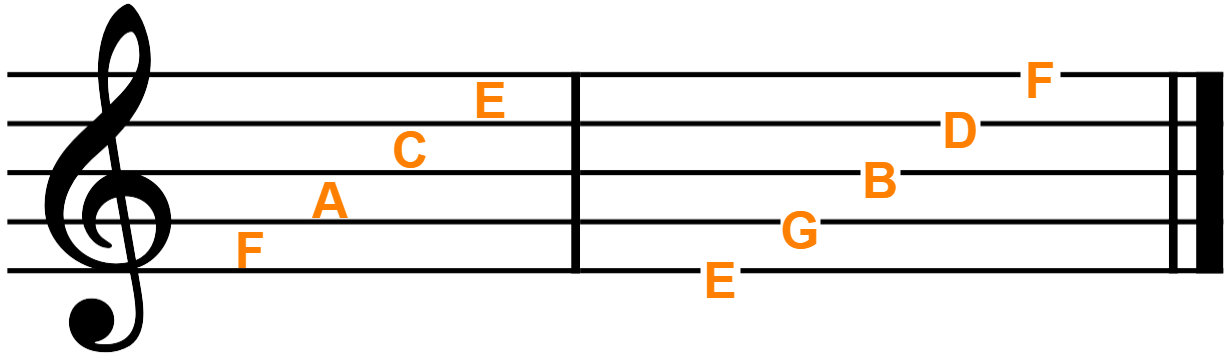
\includegraphics[width=0.6\textwidth]{../../Images/MusicNotation_MeasureNoteNames.png}
	\caption{Note names on the staff in two measures}
	\label{fig:ukulele_music_note_names_on_staff}
\end{figure}

\newpage

\subsection{Time signatures}

So far we have also only seen one type of note. The quarter note. However, there are more. See \ref{fig:ukulele_note_duration_basic}. The \lilyTimeSignature{4}{4} means that there can fit 4 (top number) quarter notes (bottom number) in a measure. 

\begin{figure}[h]
	\centering
	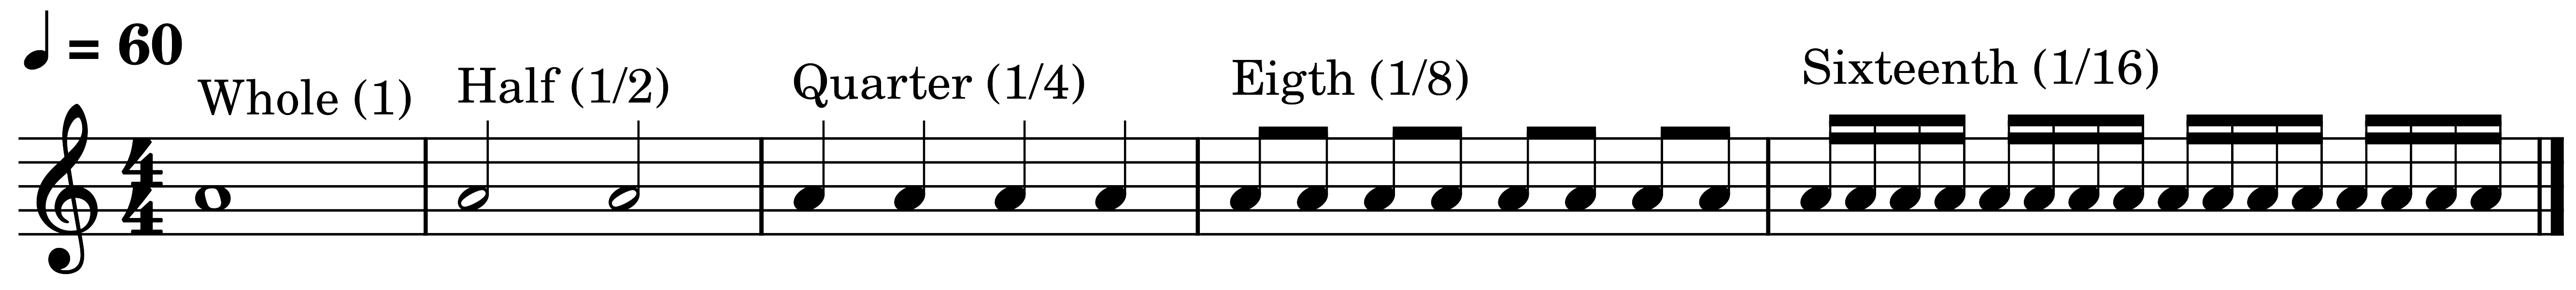
\includegraphics[width=\textwidth]{../../MuseScore/Ukulele/MusicNotation/NoteDurations_Basic.png}
	\caption{Note duration}
	\label{fig:ukulele_note_duration_basic}
\end{figure}

\textbf{Important}: A whole note (\wholeNote) equal 4 quarter notes (\quarterNote). It does \textbf{not} equal a whole measure. \newline

There are also other time signatures. But they all have the meaning. The top value indicated how many notes of the bottom number's duration fit in a measure. So a \lilyTimeSignature{3}{4} time signature can fit 3 quarter notes per measure. And a \lilyTimeSignature{6}{8} time signature can fit 6 eight notes per measure. Note that \lilyTimeSignature{3}{4} and \lilyTimeSignature{6}{8} actually indicate the same duration per measure, but they indicate a different feel. This is indicated in \ref{fig:time_signatures}

In \ref{fig:ukulele_time_signatures} you also see a new duration notation. In the first measure with \lilyTimeSignature{6}{8} timing, there are dots next to the notes (\quarterNoteDottedDown). This means that the note has a duration of 1.5x its original duration.

\begin{figure}[h]
	\centering
	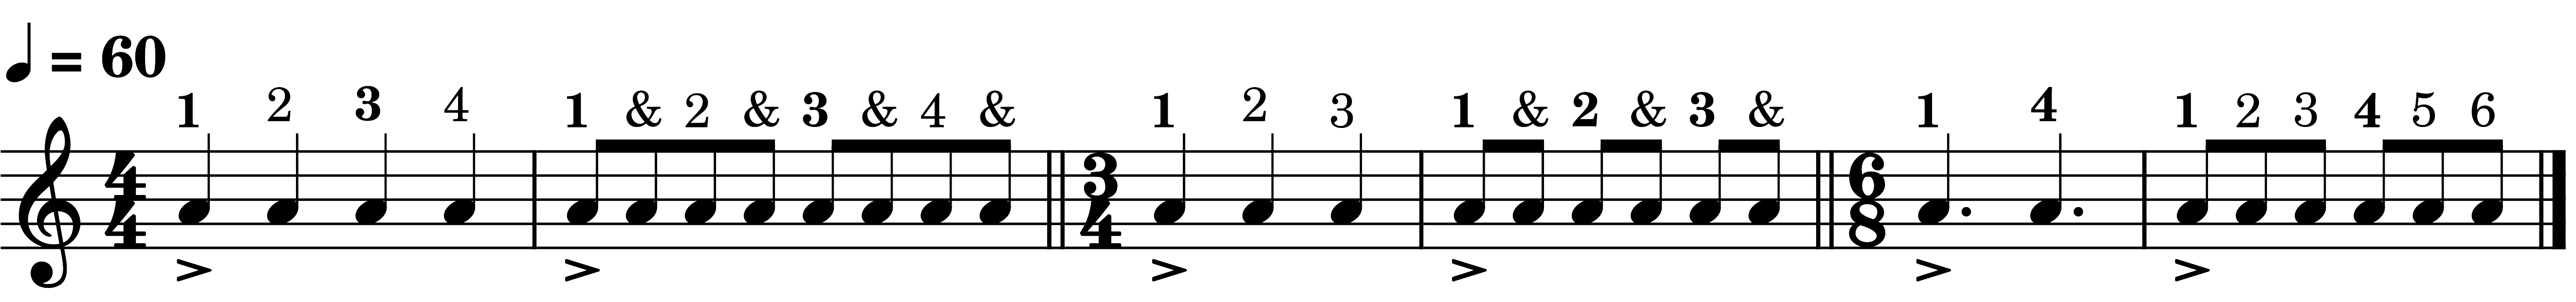
\includegraphics[width=\textwidth]{../../MuseScore/Ukulele/MusicNotation/TimeSignature.png}
	\caption{Time signatures}
	\label{fig:ukulele_time_signatures}
\end{figure}

\newpage

\subsection{Exercise}

In preparation to play the well-known "Tetris" tune, the notes from \ref{fig:ukulele_notes_for_tetris_first_part} should be learned.

\begin{figure}[h]
	\centering
	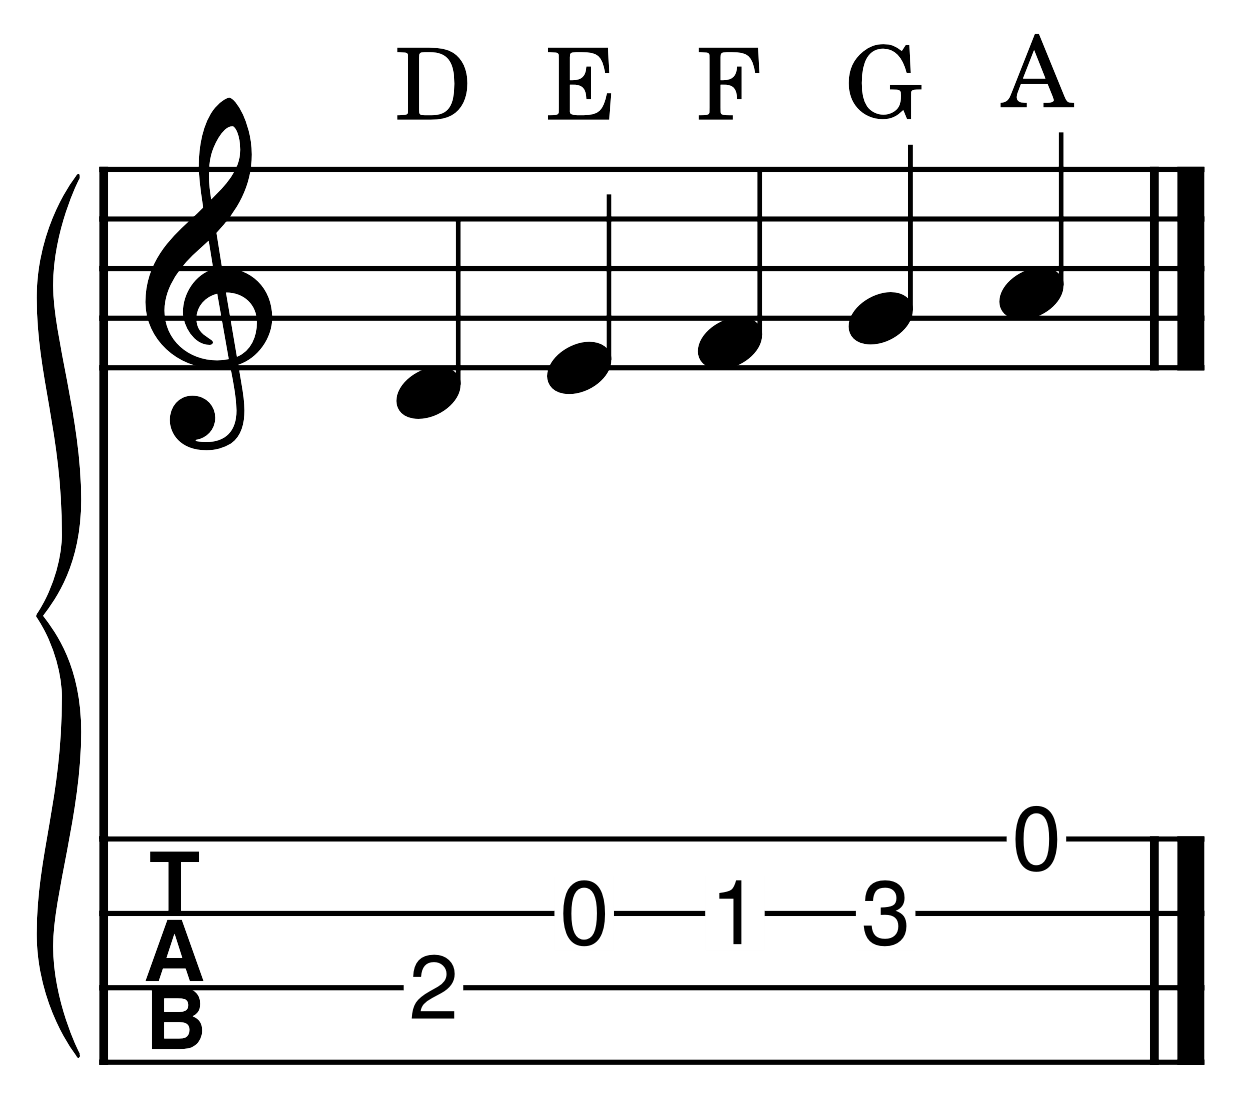
\includegraphics[width=0.25\textwidth]{../../MuseScore/Ukulele/UkuleleNotesUsedInTetrisFirstPart.png}
	\caption{Notes used for the first part of the Tetris tune}
	\label{fig:ukulele_notes_for_tetris_first_part}
\end{figure}

In \ref{fig:ukulele_tetris_simple_first_part} the first part of the Tetris tune is written. This time no TABs are shown. This exercise has 4 different note durations and 5 different notes pitches.

\begin{figure}[h]
	\centering
	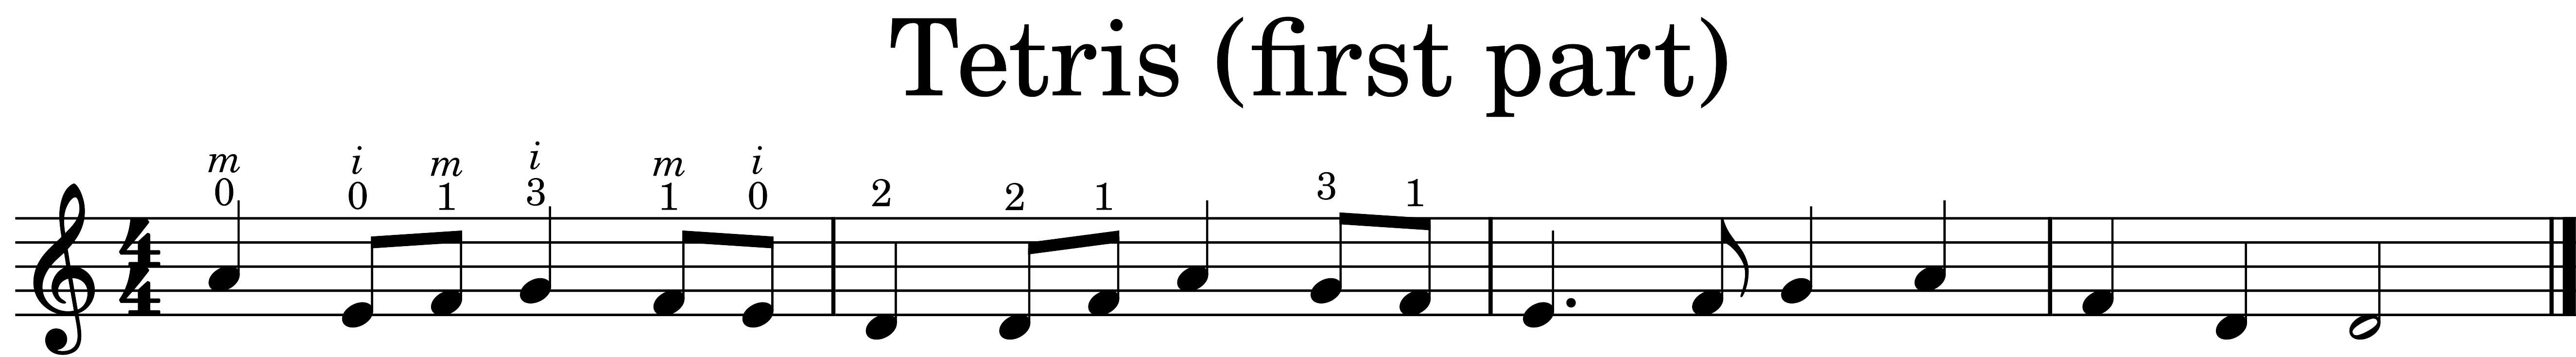
\includegraphics[width=\textwidth]{../../MuseScore/Ukulele/UkuleleTetrisSimpleFirstPart.png}
	\caption{First part of the Tetris tune}
	\label{fig:ukulele_tetris_simple_first_part}
\end{figure}


\infobox{The "Tetris" tune is actually derived from a Russian folk song called "Korobeiniki", which is based the a similar named poem written by Nikolai Nekrasov.}
\newpage
\chapter{Music notation}

\section{Music notation anatomy}

\subsection{Note names}

You have already seen the music staff from \ref{fig:ukulele_music_note_names_on_staff} in the previous exercises. However, the meaning of it was not explained yet.

The letters A-G on the staff show which line on the staff has which note value. The notes that are in between the lines nicely spell out "FACE", making it easy to remember. The Note that are on the lines can be remembered with the mnemonic "\textbf{E}very \textbf{G}ood \textbf{B}oy \textbf{D}oes \textbf{F}ine". But another important thing to see is that the notes go up alphabetically (starting again with A after G). 

The most left symbol (\clefG) is called the G clef. Note that the curl of the G clef is on the line of the G note. 

The vertical line in the middle indicates the start/end of a new measure. and the thinner vertical line in at the end indicates the end of the piece.

\begin{figure}[h]
	\centering
	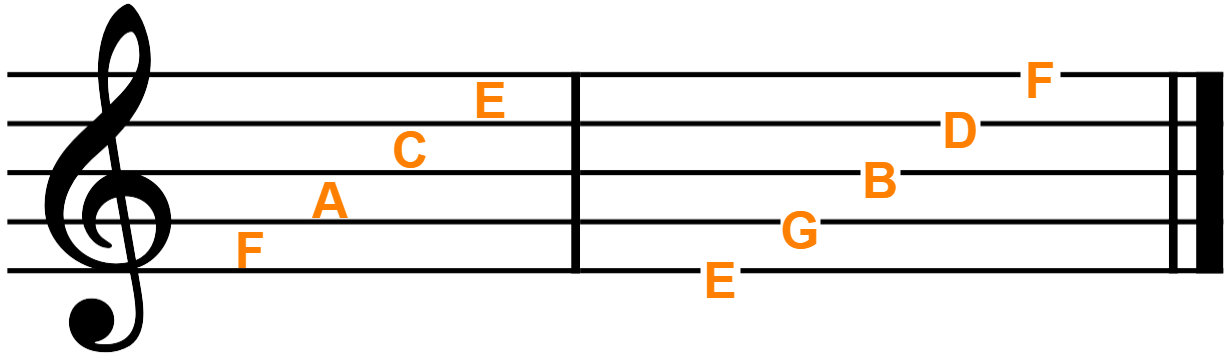
\includegraphics[width=0.6\textwidth]{../../Images/MusicNotation_MeasureNoteNames.png}
	\caption{Note names on the staff in two measures}
	\label{fig:ukulele_music_note_names_on_staff}
\end{figure}

\newpage

\subsection{Time signatures}

So far we have also only seen one type of note. The quarter note. However, there are more. See \ref{fig:ukulele_note_duration_basic}. The \lilyTimeSignature{4}{4} means that there can fit 4 (top number) quarter notes (bottom number) in a measure. 

\begin{figure}[h]
	\centering
	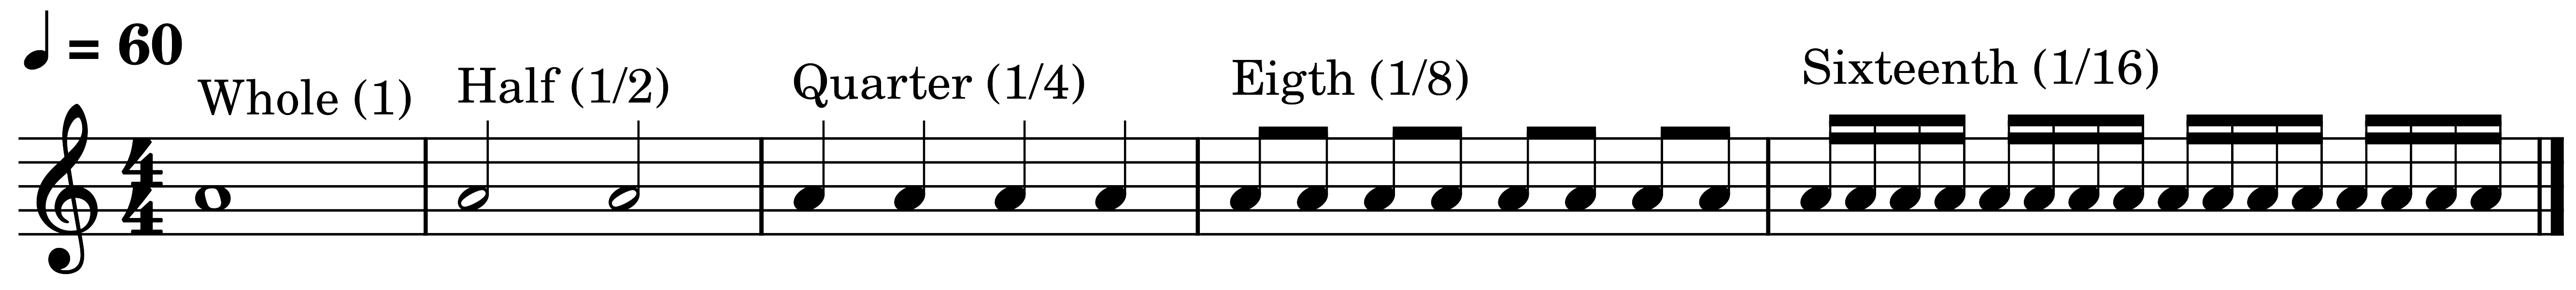
\includegraphics[width=\textwidth]{../../MuseScore/Ukulele/MusicNotation/NoteDurations_Basic.png}
	\caption{Note duration}
	\label{fig:ukulele_note_duration_basic}
\end{figure}

\textbf{Important}: A whole note (\wholeNote) equal 4 quarter notes (\quarterNote). It does \textbf{not} equal a whole measure. \newline

There are also other time signatures. But they all have the meaning. The top value indicated how many notes of the bottom number's duration fit in a measure. So a \lilyTimeSignature{3}{4} time signature can fit 3 quarter notes per measure. And a \lilyTimeSignature{6}{8} time signature can fit 6 eight notes per measure. Note that \lilyTimeSignature{3}{4} and \lilyTimeSignature{6}{8} actually indicate the same duration per measure, but they indicate a different feel. This is indicated in \ref{fig:time_signatures}

In \ref{fig:ukulele_time_signatures} you also see a new duration notation. In the first measure with \lilyTimeSignature{6}{8} timing, there are dots next to the notes (\quarterNoteDottedDown). This means that the note has a duration of 1.5x its original duration.

\begin{figure}[h]
	\centering
	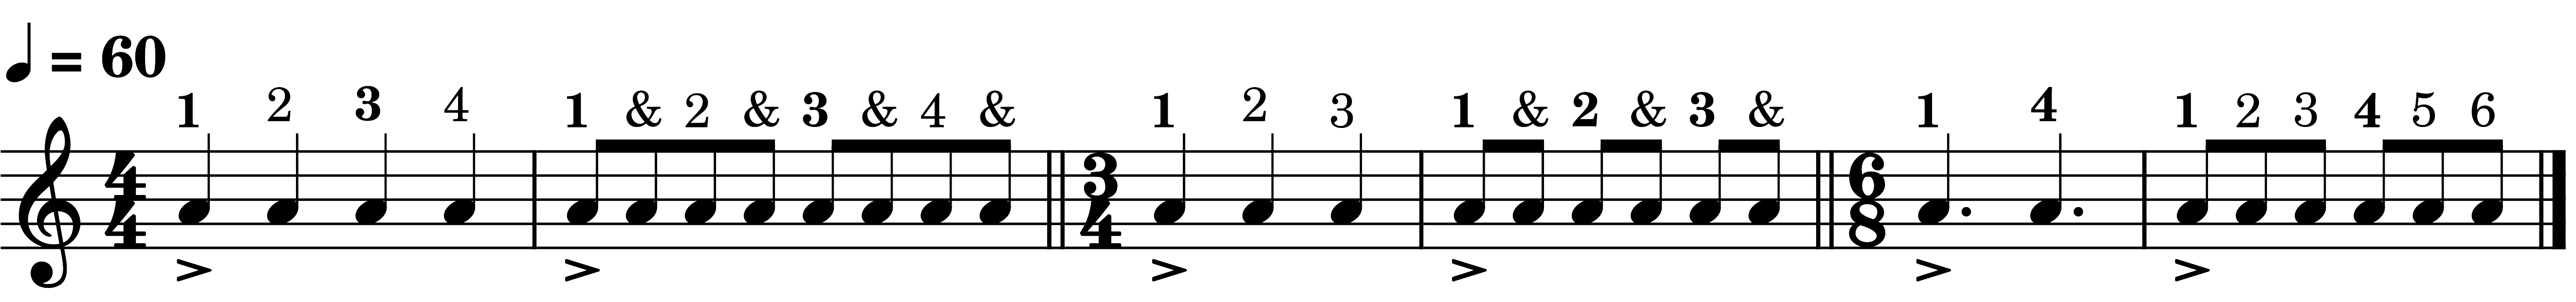
\includegraphics[width=\textwidth]{../../MuseScore/Ukulele/MusicNotation/TimeSignature.png}
	\caption{Time signatures}
	\label{fig:ukulele_time_signatures}
\end{figure}

\newpage

\subsection{Exercise}

In preparation to play the well-known "Tetris" tune, the notes from \ref{fig:ukulele_notes_for_tetris_first_part} should be learned.

\begin{figure}[h]
	\centering
	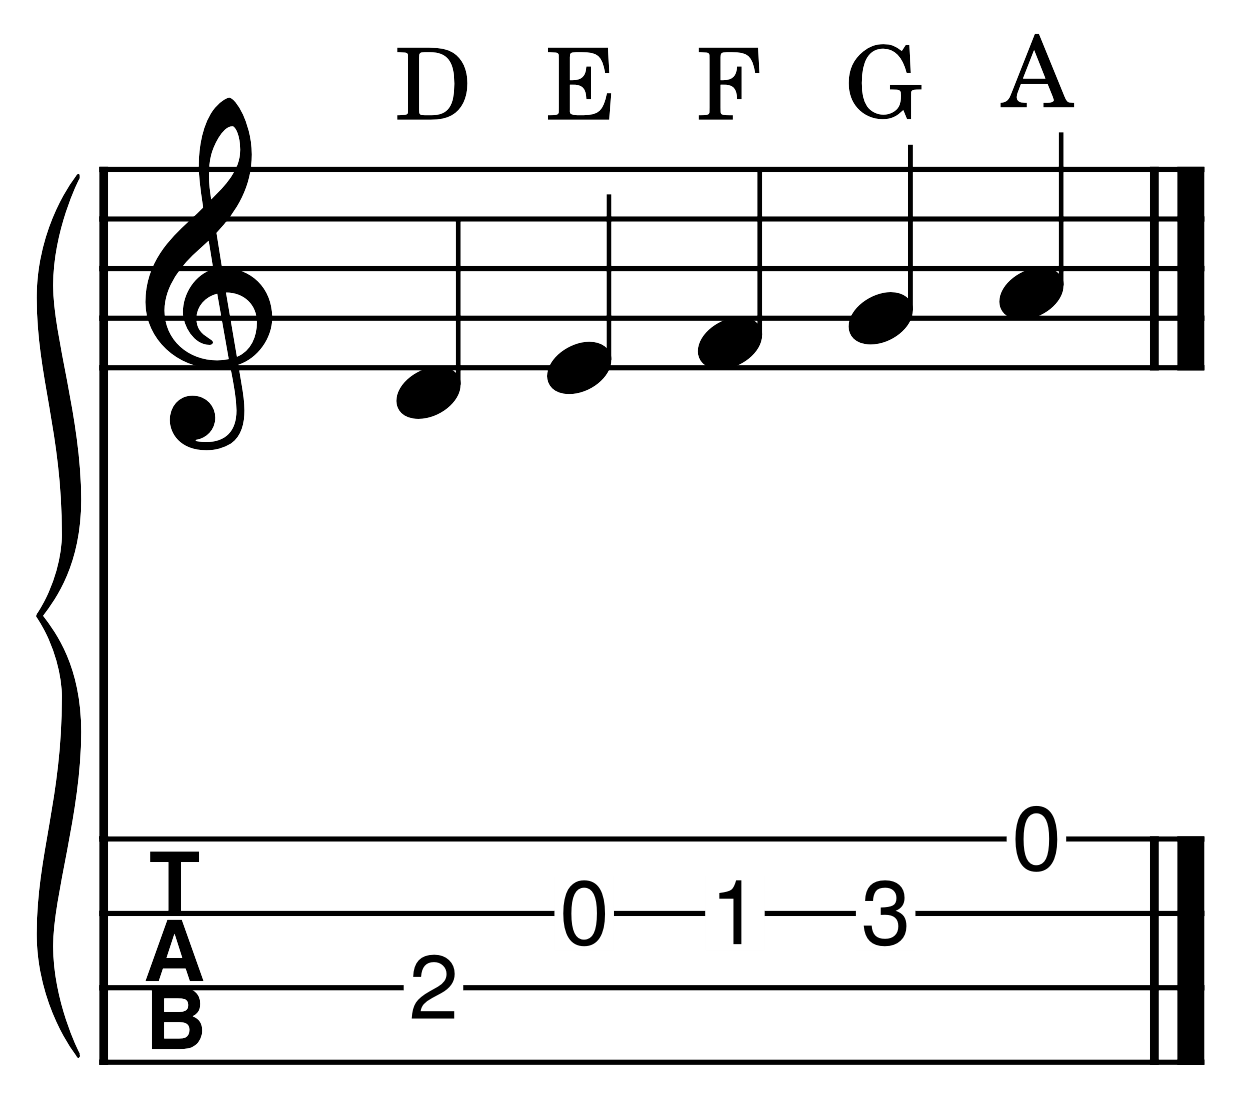
\includegraphics[width=0.25\textwidth]{../../MuseScore/Ukulele/UkuleleNotesUsedInTetrisFirstPart.png}
	\caption{Notes used for the first part of the Tetris tune}
	\label{fig:ukulele_notes_for_tetris_first_part}
\end{figure}

In \ref{fig:ukulele_tetris_simple_first_part} the first part of the Tetris tune is written. This time no TABs are shown. This exercise has 4 different note durations and 5 different notes pitches.

\begin{figure}[h]
	\centering
	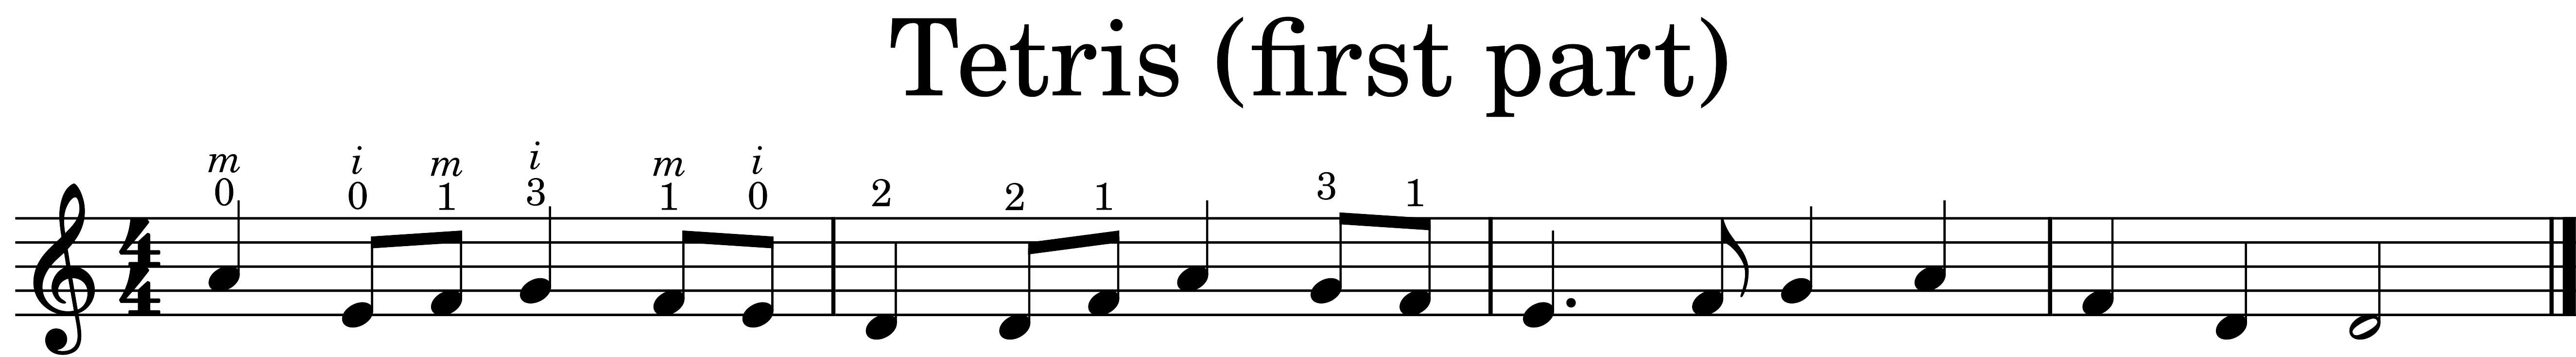
\includegraphics[width=\textwidth]{../../MuseScore/Ukulele/UkuleleTetrisSimpleFirstPart.png}
	\caption{First part of the Tetris tune}
	\label{fig:ukulele_tetris_simple_first_part}
\end{figure}


\infobox{The "Tetris" tune is actually derived from a Russian folk song called "Korobeiniki", which is based the a similar named poem written by Nikolai Nekrasov.}

\part{Ukulele}
\chapter{Music notation}

\section{Music notation anatomy}

\subsection{Note names}

You have already seen the music staff from \ref{fig:ukulele_music_note_names_on_staff} in the previous exercises. However, the meaning of it was not explained yet.

The letters A-G on the staff show which line on the staff has which note value. The notes that are in between the lines nicely spell out "FACE", making it easy to remember. The Note that are on the lines can be remembered with the mnemonic "\textbf{E}very \textbf{G}ood \textbf{B}oy \textbf{D}oes \textbf{F}ine". But another important thing to see is that the notes go up alphabetically (starting again with A after G). 

The most left symbol (\clefG) is called the G clef. Note that the curl of the G clef is on the line of the G note. 

The vertical line in the middle indicates the start/end of a new measure. and the thinner vertical line in at the end indicates the end of the piece.

\begin{figure}[h]
	\centering
	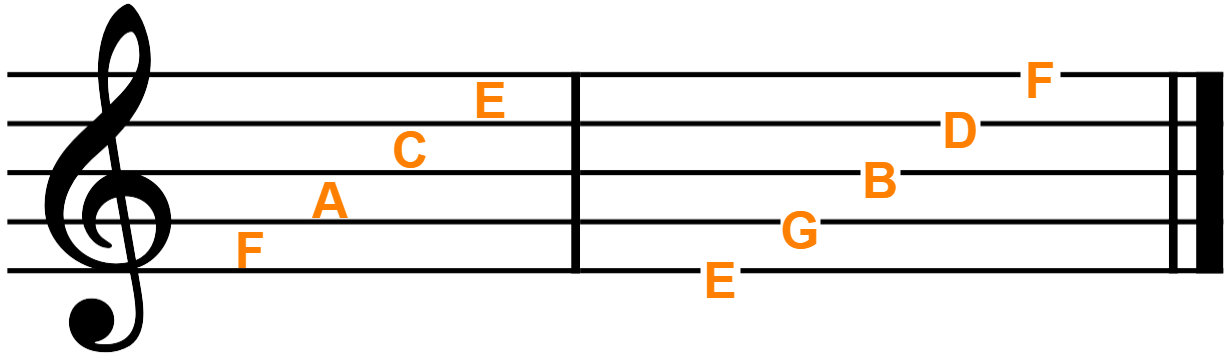
\includegraphics[width=0.6\textwidth]{../../Images/MusicNotation_MeasureNoteNames.png}
	\caption{Note names on the staff in two measures}
	\label{fig:ukulele_music_note_names_on_staff}
\end{figure}

\newpage

\subsection{Time signatures}

So far we have also only seen one type of note. The quarter note. However, there are more. See \ref{fig:ukulele_note_duration_basic}. The \lilyTimeSignature{4}{4} means that there can fit 4 (top number) quarter notes (bottom number) in a measure. 

\begin{figure}[h]
	\centering
	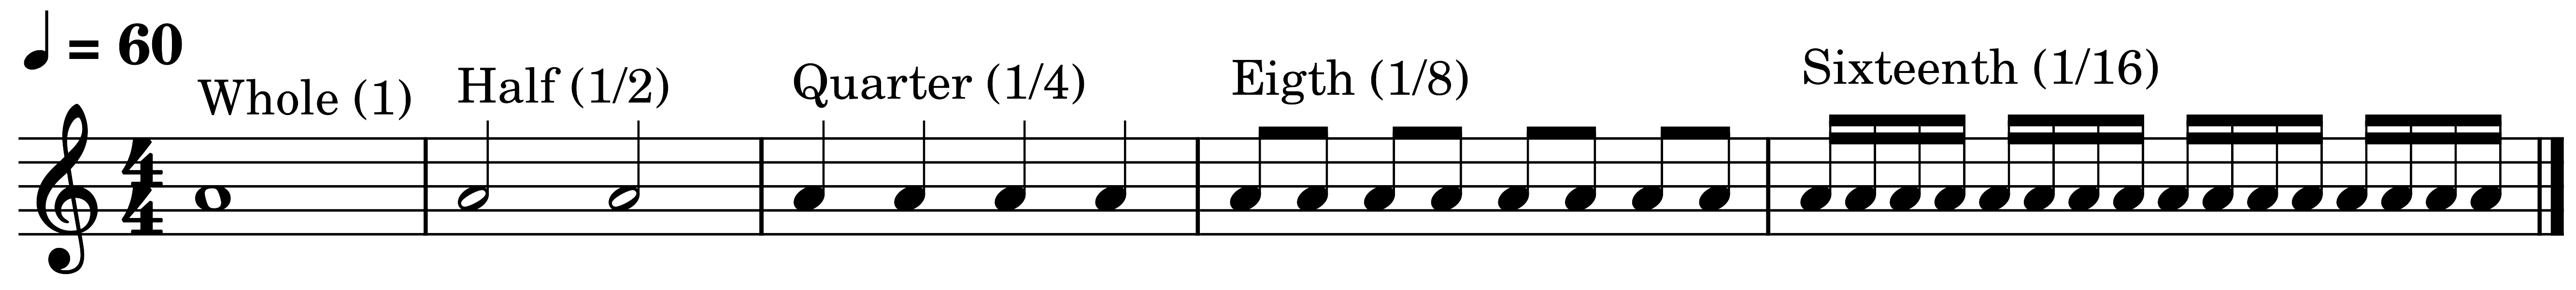
\includegraphics[width=\textwidth]{../../MuseScore/Ukulele/MusicNotation/NoteDurations_Basic.png}
	\caption{Note duration}
	\label{fig:ukulele_note_duration_basic}
\end{figure}

\textbf{Important}: A whole note (\wholeNote) equal 4 quarter notes (\quarterNote). It does \textbf{not} equal a whole measure. \newline

There are also other time signatures. But they all have the meaning. The top value indicated how many notes of the bottom number's duration fit in a measure. So a \lilyTimeSignature{3}{4} time signature can fit 3 quarter notes per measure. And a \lilyTimeSignature{6}{8} time signature can fit 6 eight notes per measure. Note that \lilyTimeSignature{3}{4} and \lilyTimeSignature{6}{8} actually indicate the same duration per measure, but they indicate a different feel. This is indicated in \ref{fig:time_signatures}

In \ref{fig:ukulele_time_signatures} you also see a new duration notation. In the first measure with \lilyTimeSignature{6}{8} timing, there are dots next to the notes (\quarterNoteDottedDown). This means that the note has a duration of 1.5x its original duration.

\begin{figure}[h]
	\centering
	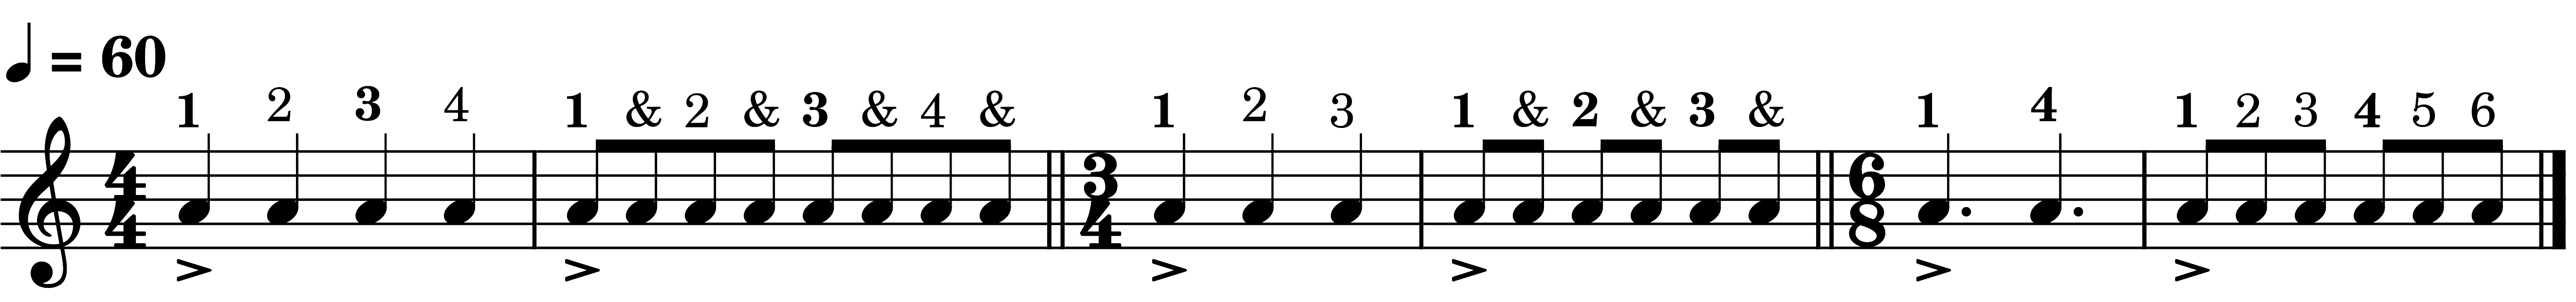
\includegraphics[width=\textwidth]{../../MuseScore/Ukulele/MusicNotation/TimeSignature.png}
	\caption{Time signatures}
	\label{fig:ukulele_time_signatures}
\end{figure}

\newpage

\subsection{Exercise}

In preparation to play the well-known "Tetris" tune, the notes from \ref{fig:ukulele_notes_for_tetris_first_part} should be learned.

\begin{figure}[h]
	\centering
	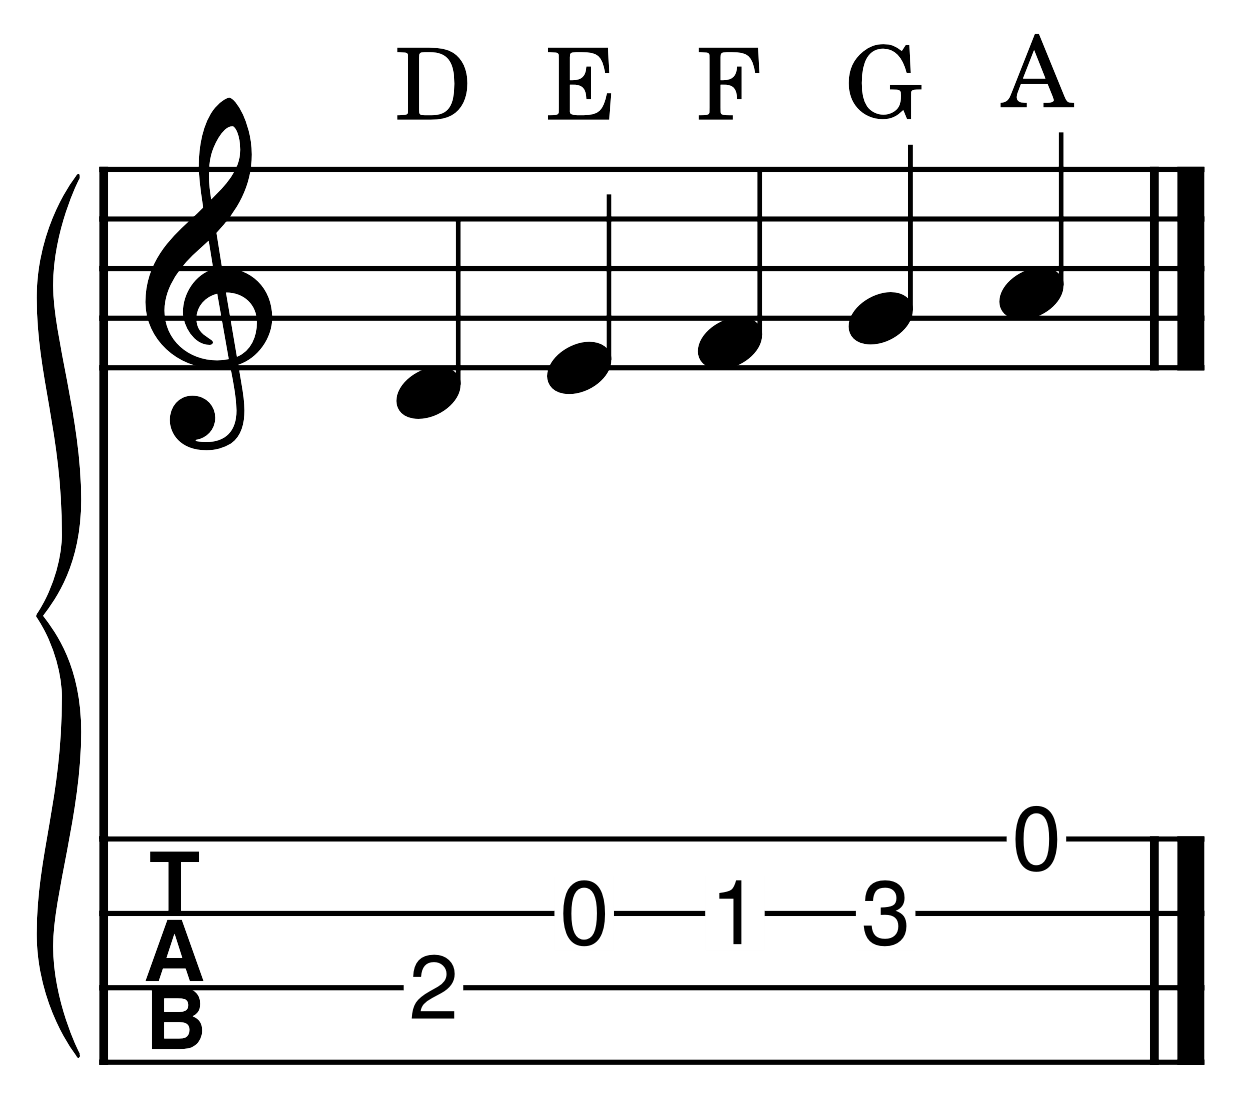
\includegraphics[width=0.25\textwidth]{../../MuseScore/Ukulele/UkuleleNotesUsedInTetrisFirstPart.png}
	\caption{Notes used for the first part of the Tetris tune}
	\label{fig:ukulele_notes_for_tetris_first_part}
\end{figure}

In \ref{fig:ukulele_tetris_simple_first_part} the first part of the Tetris tune is written. This time no TABs are shown. This exercise has 4 different note durations and 5 different notes pitches.

\begin{figure}[h]
	\centering
	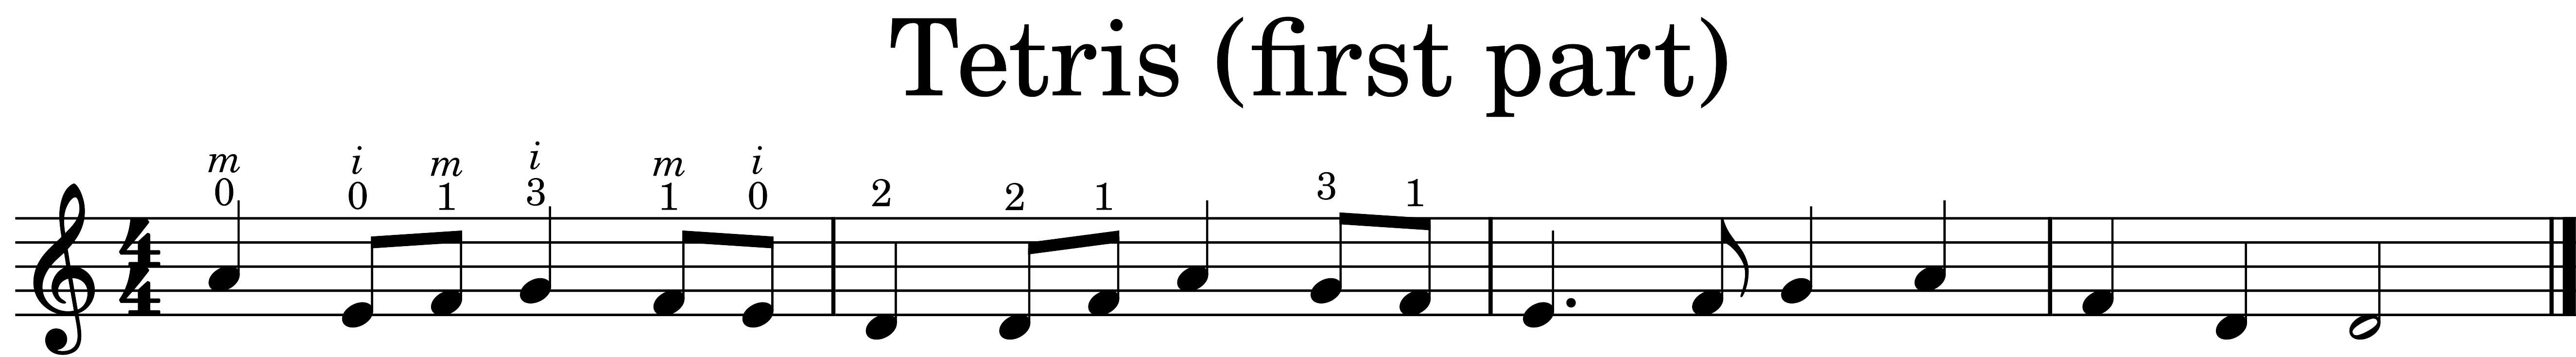
\includegraphics[width=\textwidth]{../../MuseScore/Ukulele/UkuleleTetrisSimpleFirstPart.png}
	\caption{First part of the Tetris tune}
	\label{fig:ukulele_tetris_simple_first_part}
\end{figure}


\infobox{The "Tetris" tune is actually derived from a Russian folk song called "Korobeiniki", which is based the a similar named poem written by Nikolai Nekrasov.}
\newpage
\chapter{Music notation}

\section{Music notation anatomy}

\subsection{Note names}

You have already seen the music staff from \ref{fig:ukulele_music_note_names_on_staff} in the previous exercises. However, the meaning of it was not explained yet.

The letters A-G on the staff show which line on the staff has which note value. The notes that are in between the lines nicely spell out "FACE", making it easy to remember. The Note that are on the lines can be remembered with the mnemonic "\textbf{E}very \textbf{G}ood \textbf{B}oy \textbf{D}oes \textbf{F}ine". But another important thing to see is that the notes go up alphabetically (starting again with A after G). 

The most left symbol (\clefG) is called the G clef. Note that the curl of the G clef is on the line of the G note. 

The vertical line in the middle indicates the start/end of a new measure. and the thinner vertical line in at the end indicates the end of the piece.

\begin{figure}[h]
	\centering
	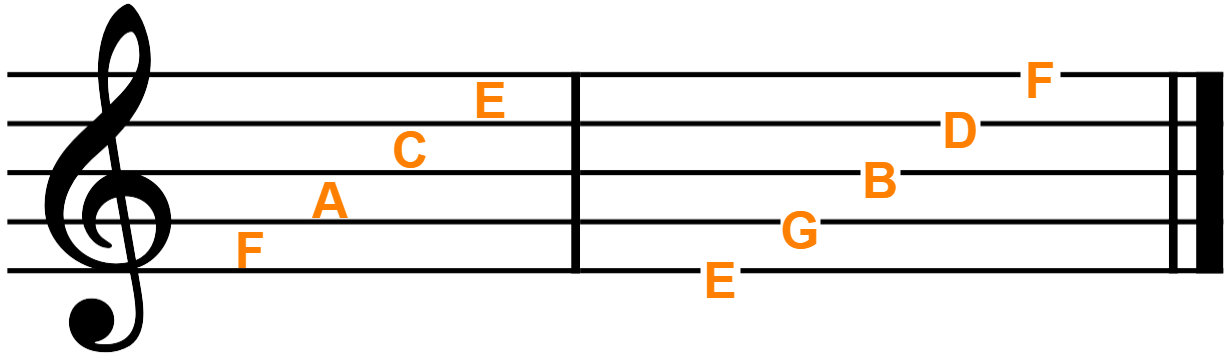
\includegraphics[width=0.6\textwidth]{../../Images/MusicNotation_MeasureNoteNames.png}
	\caption{Note names on the staff in two measures}
	\label{fig:ukulele_music_note_names_on_staff}
\end{figure}

\newpage

\subsection{Time signatures}

So far we have also only seen one type of note. The quarter note. However, there are more. See \ref{fig:ukulele_note_duration_basic}. The \lilyTimeSignature{4}{4} means that there can fit 4 (top number) quarter notes (bottom number) in a measure. 

\begin{figure}[h]
	\centering
	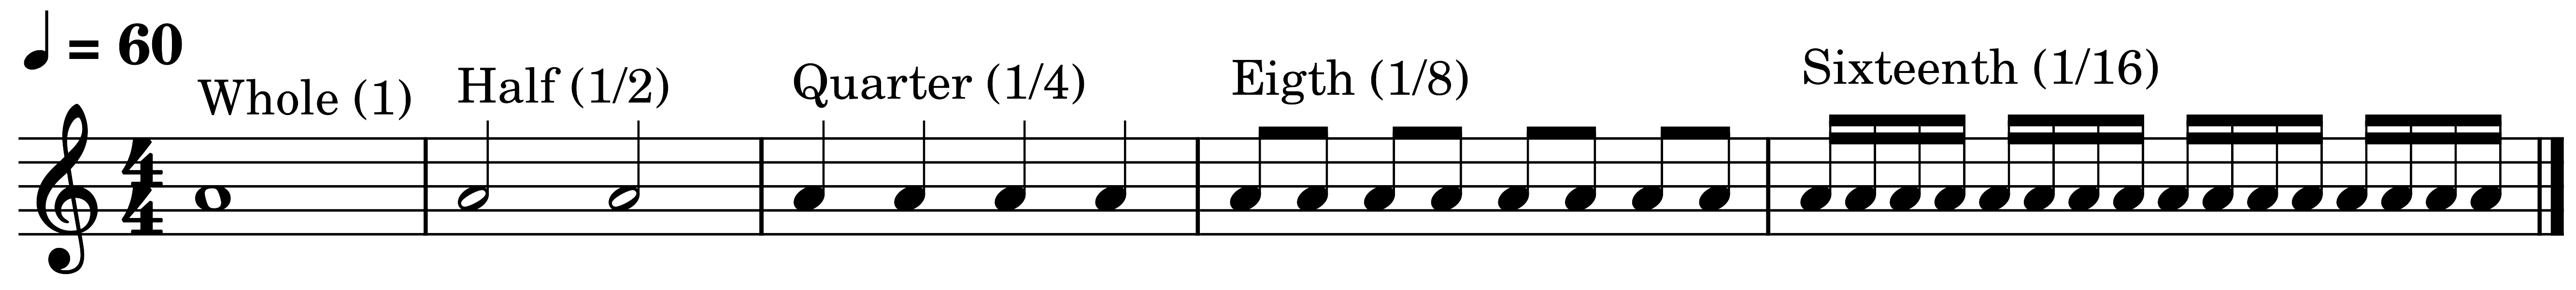
\includegraphics[width=\textwidth]{../../MuseScore/Ukulele/MusicNotation/NoteDurations_Basic.png}
	\caption{Note duration}
	\label{fig:ukulele_note_duration_basic}
\end{figure}

\textbf{Important}: A whole note (\wholeNote) equal 4 quarter notes (\quarterNote). It does \textbf{not} equal a whole measure. \newline

There are also other time signatures. But they all have the meaning. The top value indicated how many notes of the bottom number's duration fit in a measure. So a \lilyTimeSignature{3}{4} time signature can fit 3 quarter notes per measure. And a \lilyTimeSignature{6}{8} time signature can fit 6 eight notes per measure. Note that \lilyTimeSignature{3}{4} and \lilyTimeSignature{6}{8} actually indicate the same duration per measure, but they indicate a different feel. This is indicated in \ref{fig:time_signatures}

In \ref{fig:ukulele_time_signatures} you also see a new duration notation. In the first measure with \lilyTimeSignature{6}{8} timing, there are dots next to the notes (\quarterNoteDottedDown). This means that the note has a duration of 1.5x its original duration.

\begin{figure}[h]
	\centering
	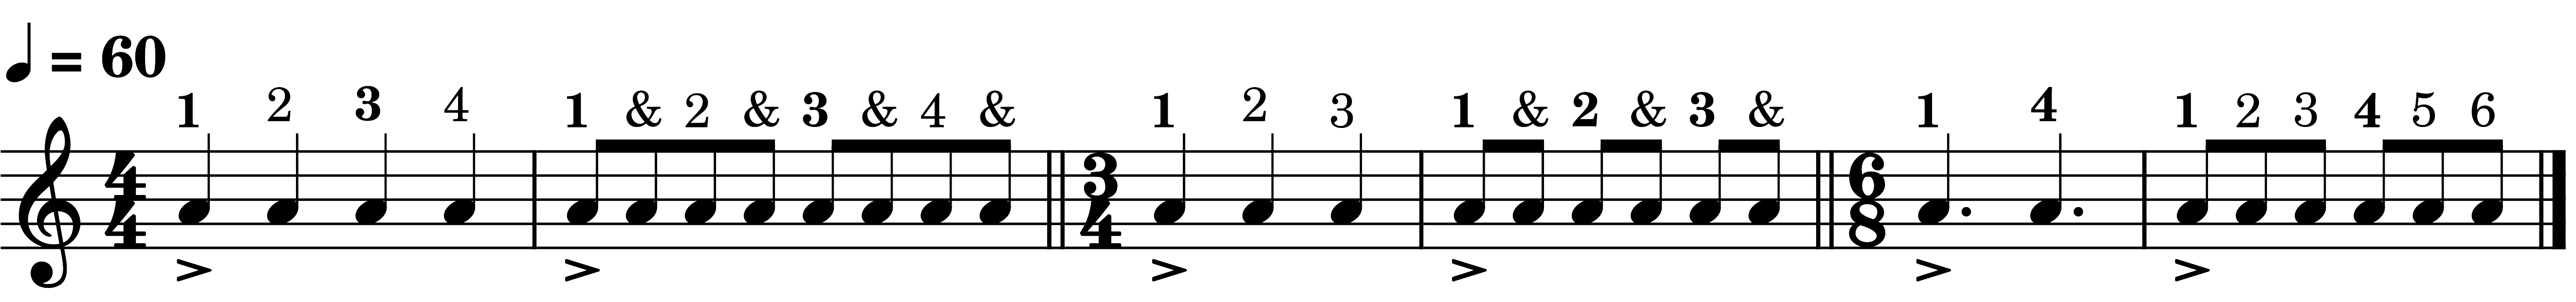
\includegraphics[width=\textwidth]{../../MuseScore/Ukulele/MusicNotation/TimeSignature.png}
	\caption{Time signatures}
	\label{fig:ukulele_time_signatures}
\end{figure}

\newpage

\subsection{Exercise}

In preparation to play the well-known "Tetris" tune, the notes from \ref{fig:ukulele_notes_for_tetris_first_part} should be learned.

\begin{figure}[h]
	\centering
	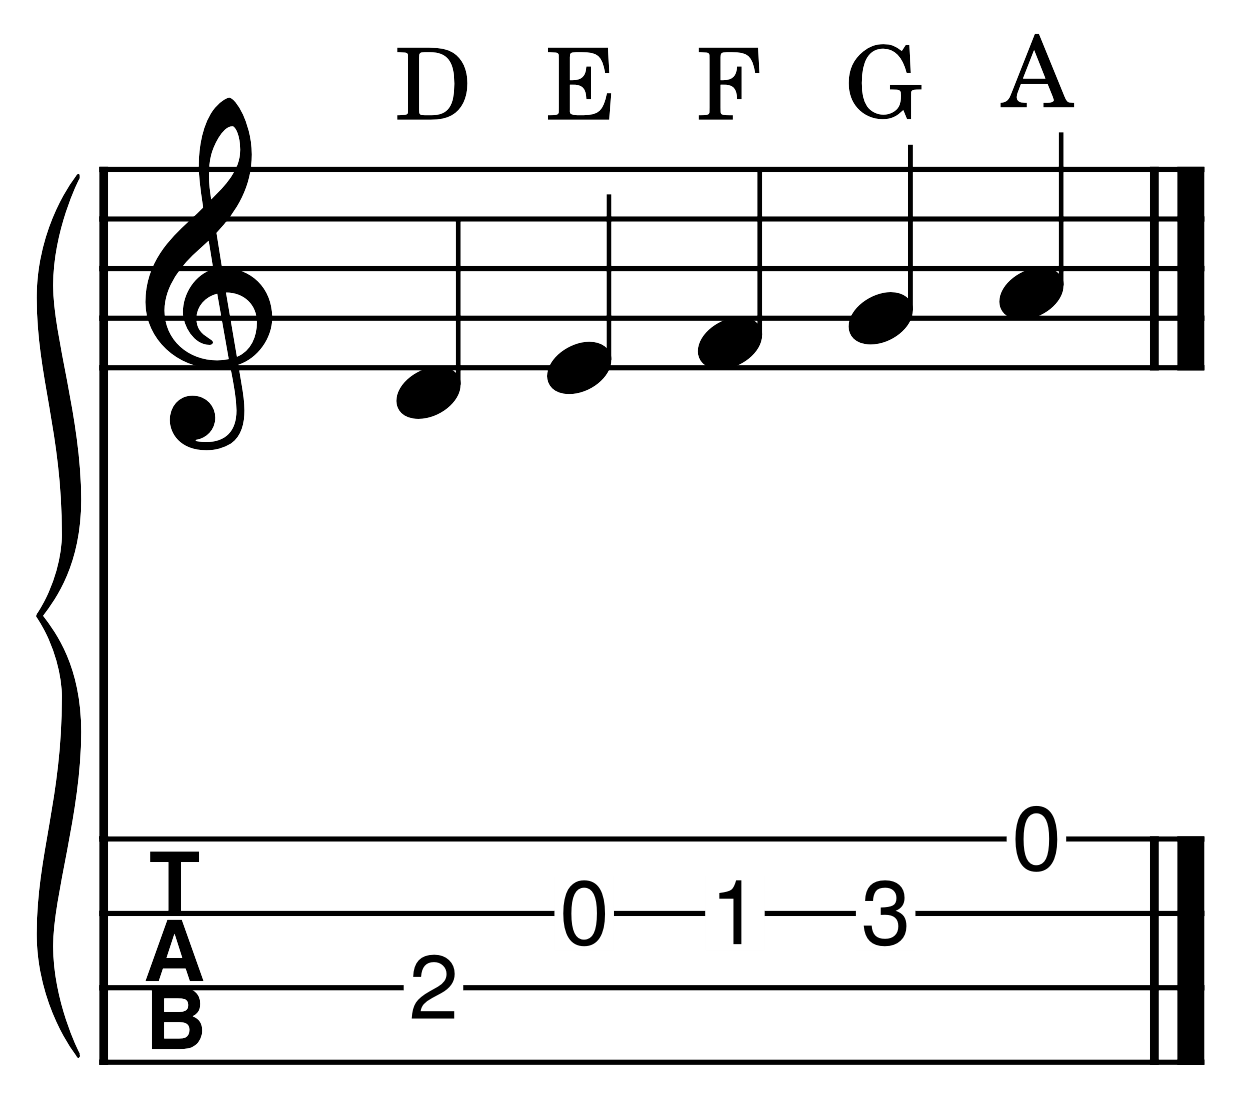
\includegraphics[width=0.25\textwidth]{../../MuseScore/Ukulele/UkuleleNotesUsedInTetrisFirstPart.png}
	\caption{Notes used for the first part of the Tetris tune}
	\label{fig:ukulele_notes_for_tetris_first_part}
\end{figure}

In \ref{fig:ukulele_tetris_simple_first_part} the first part of the Tetris tune is written. This time no TABs are shown. This exercise has 4 different note durations and 5 different notes pitches.

\begin{figure}[h]
	\centering
	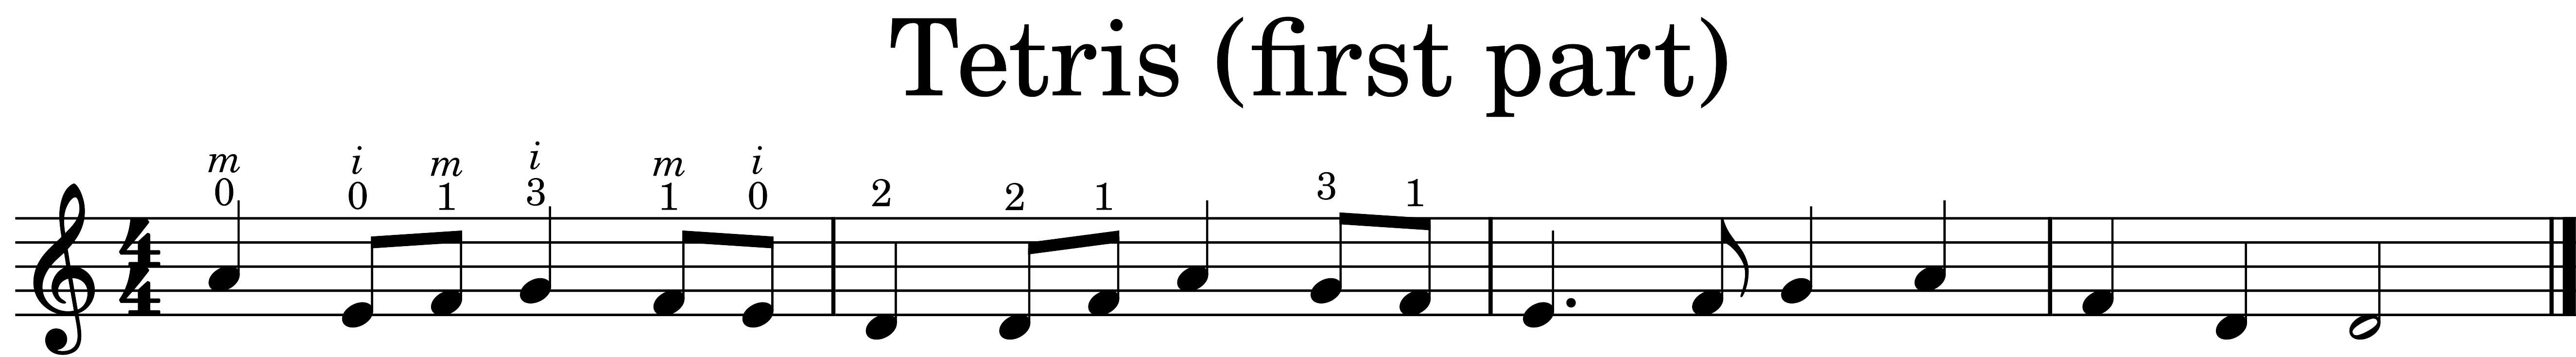
\includegraphics[width=\textwidth]{../../MuseScore/Ukulele/UkuleleTetrisSimpleFirstPart.png}
	\caption{First part of the Tetris tune}
	\label{fig:ukulele_tetris_simple_first_part}
\end{figure}


\infobox{The "Tetris" tune is actually derived from a Russian folk song called "Korobeiniki", which is based the a similar named poem written by Nikolai Nekrasov.}
\newpage
\chapter{Music notation}

\section{Music notation anatomy}

\subsection{Note names}

You have already seen the music staff from \ref{fig:ukulele_music_note_names_on_staff} in the previous exercises. However, the meaning of it was not explained yet.

The letters A-G on the staff show which line on the staff has which note value. The notes that are in between the lines nicely spell out "FACE", making it easy to remember. The Note that are on the lines can be remembered with the mnemonic "\textbf{E}very \textbf{G}ood \textbf{B}oy \textbf{D}oes \textbf{F}ine". But another important thing to see is that the notes go up alphabetically (starting again with A after G). 

The most left symbol (\clefG) is called the G clef. Note that the curl of the G clef is on the line of the G note. 

The vertical line in the middle indicates the start/end of a new measure. and the thinner vertical line in at the end indicates the end of the piece.

\begin{figure}[h]
	\centering
	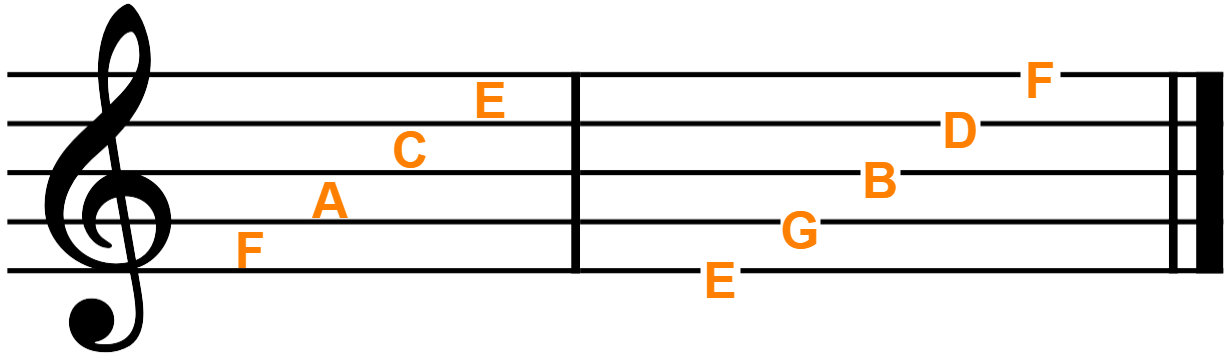
\includegraphics[width=0.6\textwidth]{../../Images/MusicNotation_MeasureNoteNames.png}
	\caption{Note names on the staff in two measures}
	\label{fig:ukulele_music_note_names_on_staff}
\end{figure}

\newpage

\subsection{Time signatures}

So far we have also only seen one type of note. The quarter note. However, there are more. See \ref{fig:ukulele_note_duration_basic}. The \lilyTimeSignature{4}{4} means that there can fit 4 (top number) quarter notes (bottom number) in a measure. 

\begin{figure}[h]
	\centering
	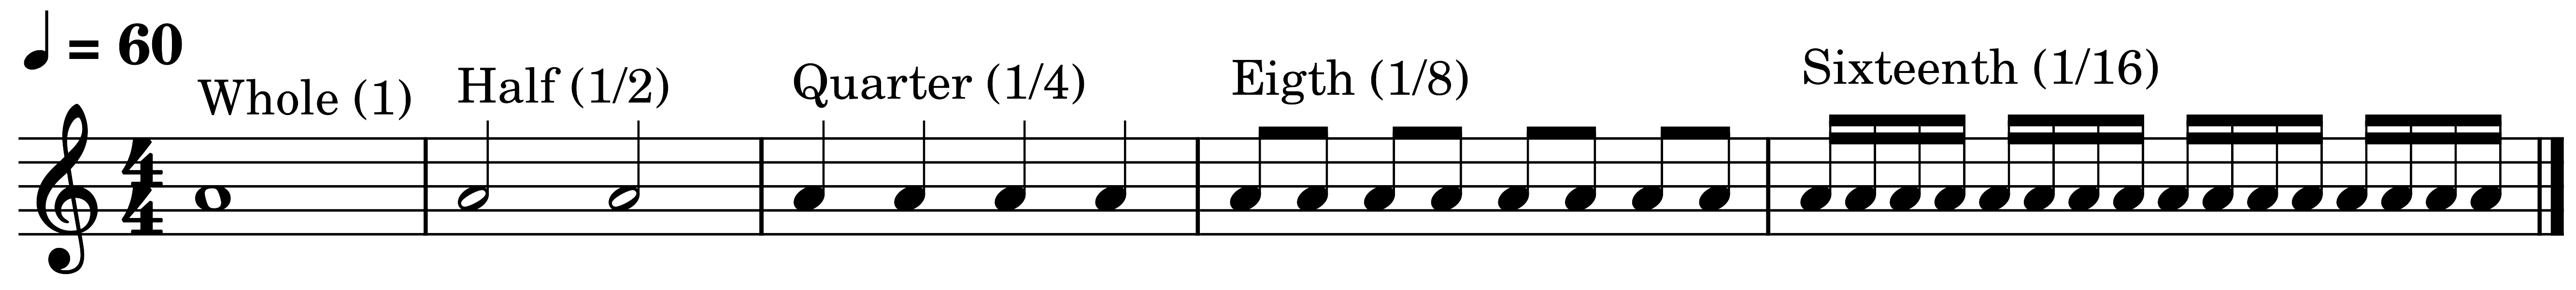
\includegraphics[width=\textwidth]{../../MuseScore/Ukulele/MusicNotation/NoteDurations_Basic.png}
	\caption{Note duration}
	\label{fig:ukulele_note_duration_basic}
\end{figure}

\textbf{Important}: A whole note (\wholeNote) equal 4 quarter notes (\quarterNote). It does \textbf{not} equal a whole measure. \newline

There are also other time signatures. But they all have the meaning. The top value indicated how many notes of the bottom number's duration fit in a measure. So a \lilyTimeSignature{3}{4} time signature can fit 3 quarter notes per measure. And a \lilyTimeSignature{6}{8} time signature can fit 6 eight notes per measure. Note that \lilyTimeSignature{3}{4} and \lilyTimeSignature{6}{8} actually indicate the same duration per measure, but they indicate a different feel. This is indicated in \ref{fig:time_signatures}

In \ref{fig:ukulele_time_signatures} you also see a new duration notation. In the first measure with \lilyTimeSignature{6}{8} timing, there are dots next to the notes (\quarterNoteDottedDown). This means that the note has a duration of 1.5x its original duration.

\begin{figure}[h]
	\centering
	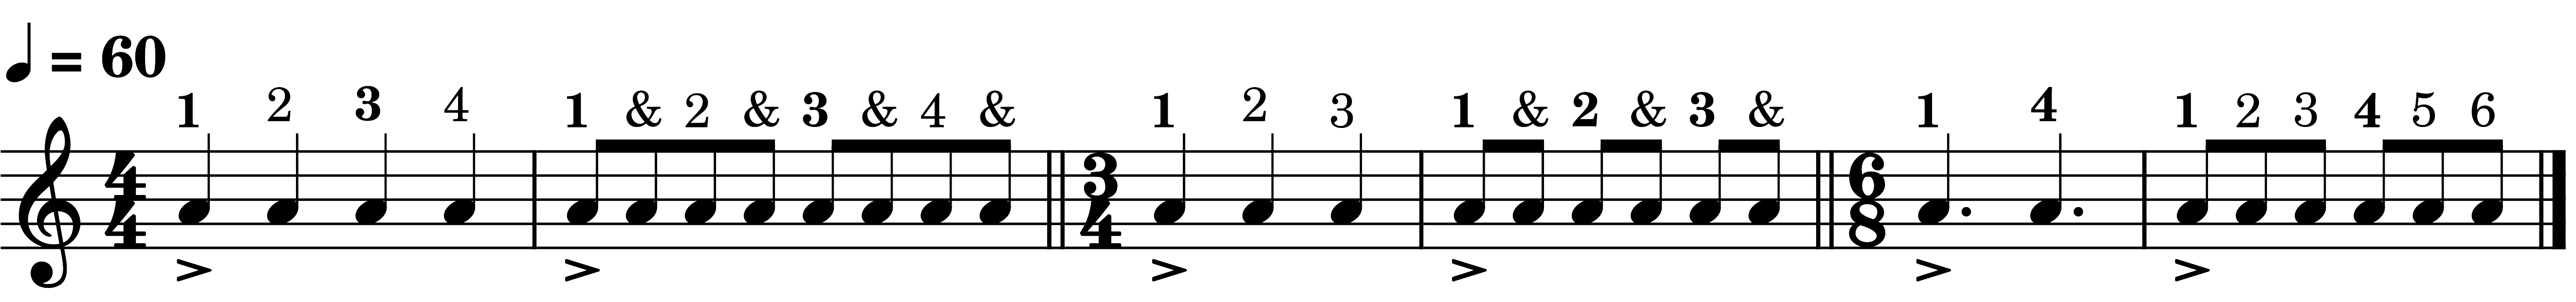
\includegraphics[width=\textwidth]{../../MuseScore/Ukulele/MusicNotation/TimeSignature.png}
	\caption{Time signatures}
	\label{fig:ukulele_time_signatures}
\end{figure}

\newpage

\subsection{Exercise}

In preparation to play the well-known "Tetris" tune, the notes from \ref{fig:ukulele_notes_for_tetris_first_part} should be learned.

\begin{figure}[h]
	\centering
	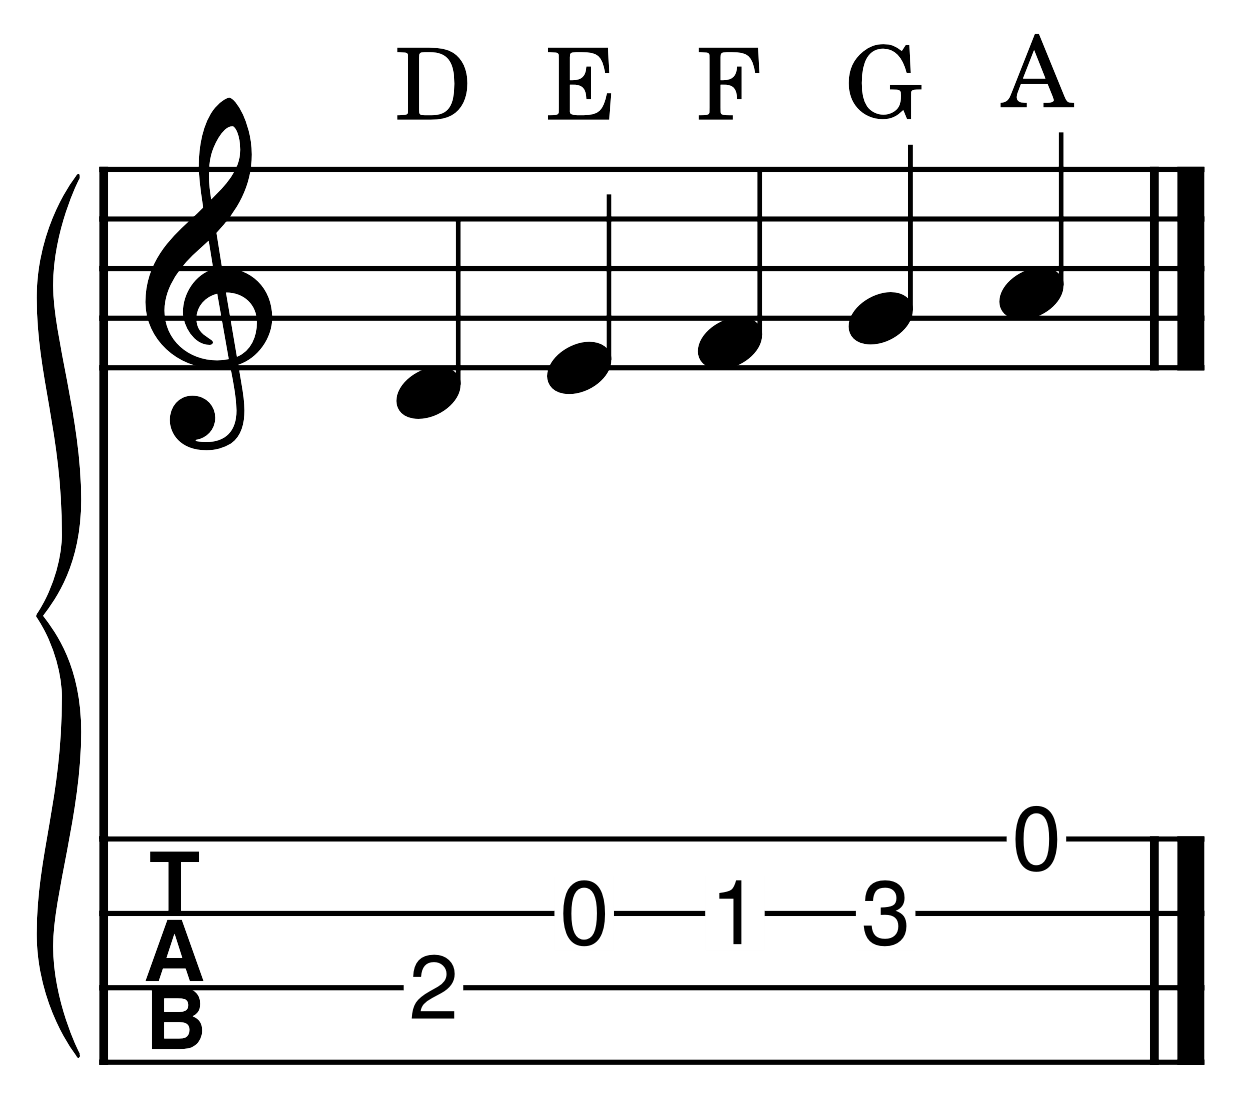
\includegraphics[width=0.25\textwidth]{../../MuseScore/Ukulele/UkuleleNotesUsedInTetrisFirstPart.png}
	\caption{Notes used for the first part of the Tetris tune}
	\label{fig:ukulele_notes_for_tetris_first_part}
\end{figure}

In \ref{fig:ukulele_tetris_simple_first_part} the first part of the Tetris tune is written. This time no TABs are shown. This exercise has 4 different note durations and 5 different notes pitches.

\begin{figure}[h]
	\centering
	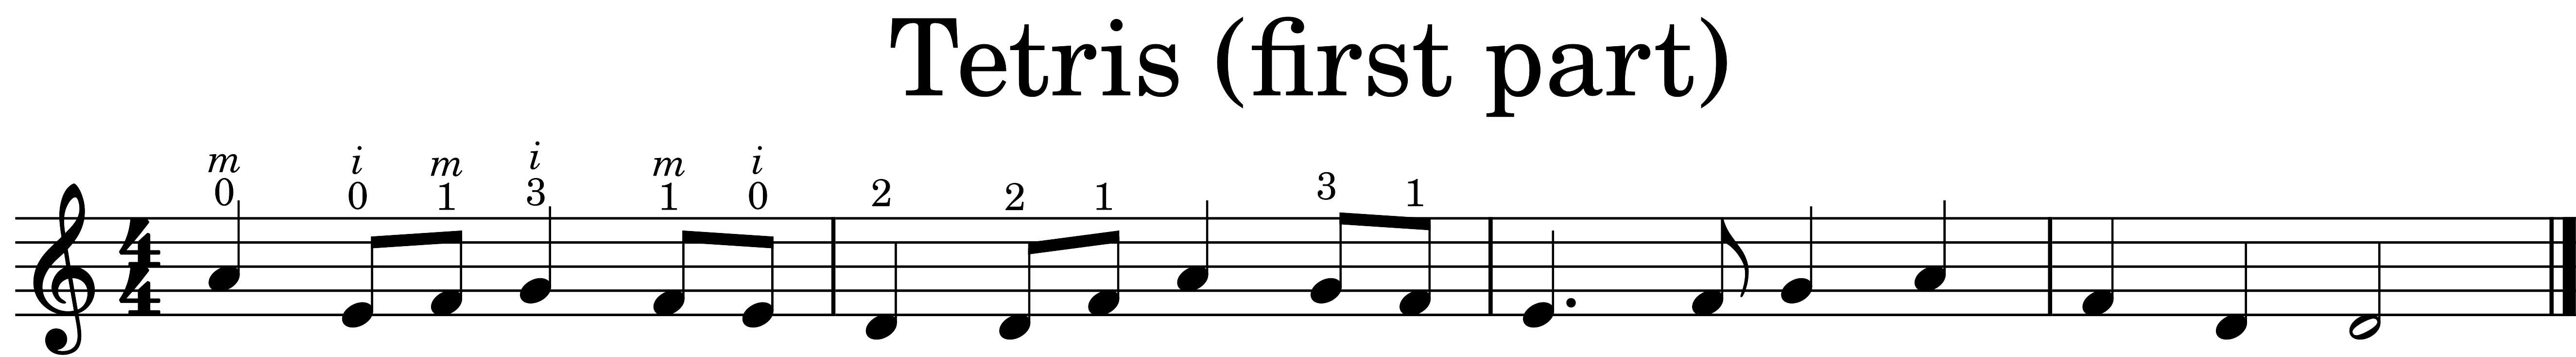
\includegraphics[width=\textwidth]{../../MuseScore/Ukulele/UkuleleTetrisSimpleFirstPart.png}
	\caption{First part of the Tetris tune}
	\label{fig:ukulele_tetris_simple_first_part}
\end{figure}


\infobox{The "Tetris" tune is actually derived from a Russian folk song called "Korobeiniki", which is based the a similar named poem written by Nikolai Nekrasov.}

%Reading notes
%Scales and Chord patterns (learning the fretboard)
%Strumming with fingers
%Basic chord shapes + CAGFD
%Extending the chords
%Finger picking
%Strumming patterns

\printbibliography

\end{document}